The SiPMs are used in the TRITIUM experiment in two different ways, at the level of a single SiPM and at the level of several SiPMs arranged in a matrix. Both studies were carried out to characterize the SiPM arrays used in the TRITIUM monitor.

The electronic system chosen to process and analyze the output signals of the SiPM arrays is PETsys \cite{PETSYS}, which is a commercial system prepared to work with SiPM matrices from Hamamatsu.

PETsys is a complete acquisition and digitization system that is capable of working with up to 1024 SiPM. This system consists of a basic board, which processes the signal, to which 16 different SiPM matrices can be connected with up to 64 SiPM per matrix. This number of channels is needed in the TRITIUM project because, as it is shown in section \ref{sec:TritiumMonitor}, the TRITIUM monitor consists of a large number of SiPM matrices with 16 channels (SiPMs) per matrix. The PETsys system used in TRITIUM is displayed in Figure \ref{fig:PETSYS}.

\begin{figure}[htbp]
\centering
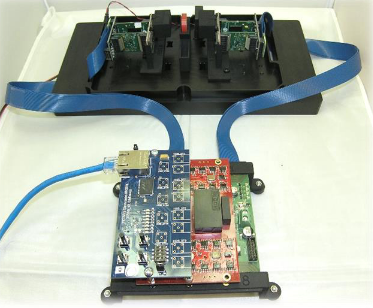
\includegraphics[scale=0.6]{3DesignPrinciples/32Tritium_detector/PETSYS_System.png}
\caption{Different parts of PETSYS system.\label{fig:PETSYS}~\cite{PETSYS}}
\end{figure}

Although the capacity provided by PETSYS should be enough for the requirements of the TRITIUM project, TRITIUM is a modular detector with scalable sensitivity. It means that, if an inprovement of its limits is needed to improve its sensitivity or to further reduce the background, more photosensors would be needed. Therefore, the electronic system should be able to increase its capacity in a scalable way. This requeriment is fulfilled by PETSYS since it has an additional module, called Clock and Trigger, to which up to sixteen different PETSYS basic boards can be connected. Theses sixteen PETsys basic boards are read in parallel, giving a total system capacity of reading 256 SiPM matrices (16384 SiPMs\footnote{$1024\cdot{}16 = 16384$}). 

PETSYS is based on C++ and Python scripts that are prepared for the main tasks required, such as time coincidence options between SiPM (or even SiPM matrices) or energy discrimination. It is open source, giving the possibility to modify the current scripts or develop others with additional functions. PETsys has a time resolution of $250~\pico\second$ which is one of the best time resolutions of commercial systems available and its price is around $10$\euro$/$ channel, which is cheaper compared to similar electronic systems.

As described in section \ref{sec:CharacterizationSiPM}, the SiPM matrix temperature is an important parameter. The PETsys system has the ability to monitor the temperature of the SiPM matrices and ASICS employed to control them. Temperature monitoring is important to ensure the correct functioning of both, photosensors and system. PETsys has the possibility of developing new function scripts to implement the stability gain method reported in section \ref{sec:CharacterizationSiPM}.

Although the TRITIUM monitor use SiPM matrices it is important to start the characterizaton at the level of a single channel (only one SiPM) to reduce the uncertainties in the first results. In order to do so, an electronic system was designed, developed and built to read up to eight different SiPMs and to monitor their temperature.

This system is based on three different PCBs\footnote{PCB, Printed Circuit Board}, shown in Figure \ref{fig:PCBs_LEDSpectrum} (electronical schemes shown in the appendix \ref{App:ElectronicalSchemesSiPMPCBs}):

\begin{enumerate}
\item{} The first PCB, shown in Figure \ref{subfig:PCB1}, is used to organize the SiPMs and sensor temperature. This PCB place up to 8 different SiPMs and a temperature sensor and arrange their output signals on two HDMI connections. This PCB is placed inside a special black box, from Thorlabs company \cite{ThorlabsCompany}, that has a high degree of light tightness. This black box has a small hole of $1~\mm$ diameter, prepared to introduce an optical fiber\footnote{The optical fiber used is BCF-98 from Saint-Gobain company \cite{OpticalFibers}} to iluminate SiPMs with an incoherent light source. The light source utilized is a LED, model 430L from Thorlabs company \cite{LEDThorlabs}, which gives an spectrum shown in Figure \ref{subfig:LEDSpectrum}. The spectrum was experimentaly measured with a spectrometer and fitted to a Gaussian function. It can be seen that the emission peak of this LED is palced at $436.3$ with a FWHM\footnote{The FWHM parameter, Full Width at Half Maximum, of a Gaussian fit can be calculated from its sigma using the equation: FWHM$=2.35 \cdot{} \sigma$} of $19.1~\nano\meter$. With the help of this LED we intend to simulate the light emission of the fibers of the TRITIUM experiment to calibrate the SiPMs at the working wavelength. 

\item{} The second PCB, shown in Figure \ref{subfig:PCB2}, sums the different signals of the SiPMs and amplify them by a factor $G=4187.5$ or $G=10761.88$, depending on the input resistance of the oscilloscope, $50~\varOmega$ or $1~\mega\varOmega$, respectively. This PCB uses a differential amplification that reduce the electronic noise of the system and is connected to the first PCB through two HDMI feedthroughs.

\item{} The third PCB, shown in Figure \ref{subfig:PCB3}, rearranges all the different input and output signals in an HDMI connection to avoid crosstalk between different signals. This PCB is connected to the second PCB trought a HDMI feedthrough.

The input signals are the supply voltage of the SiPMs and the supply voltage of the PCBs ($\pm 6~\volt$) and the output signals are the temperature sensor signal and the summed signal of all SiPMs. 

\end{enumerate}

\begin{figure}
\centering
    \begin{subfigure}[b]{0.5\textwidth}
    \centering
    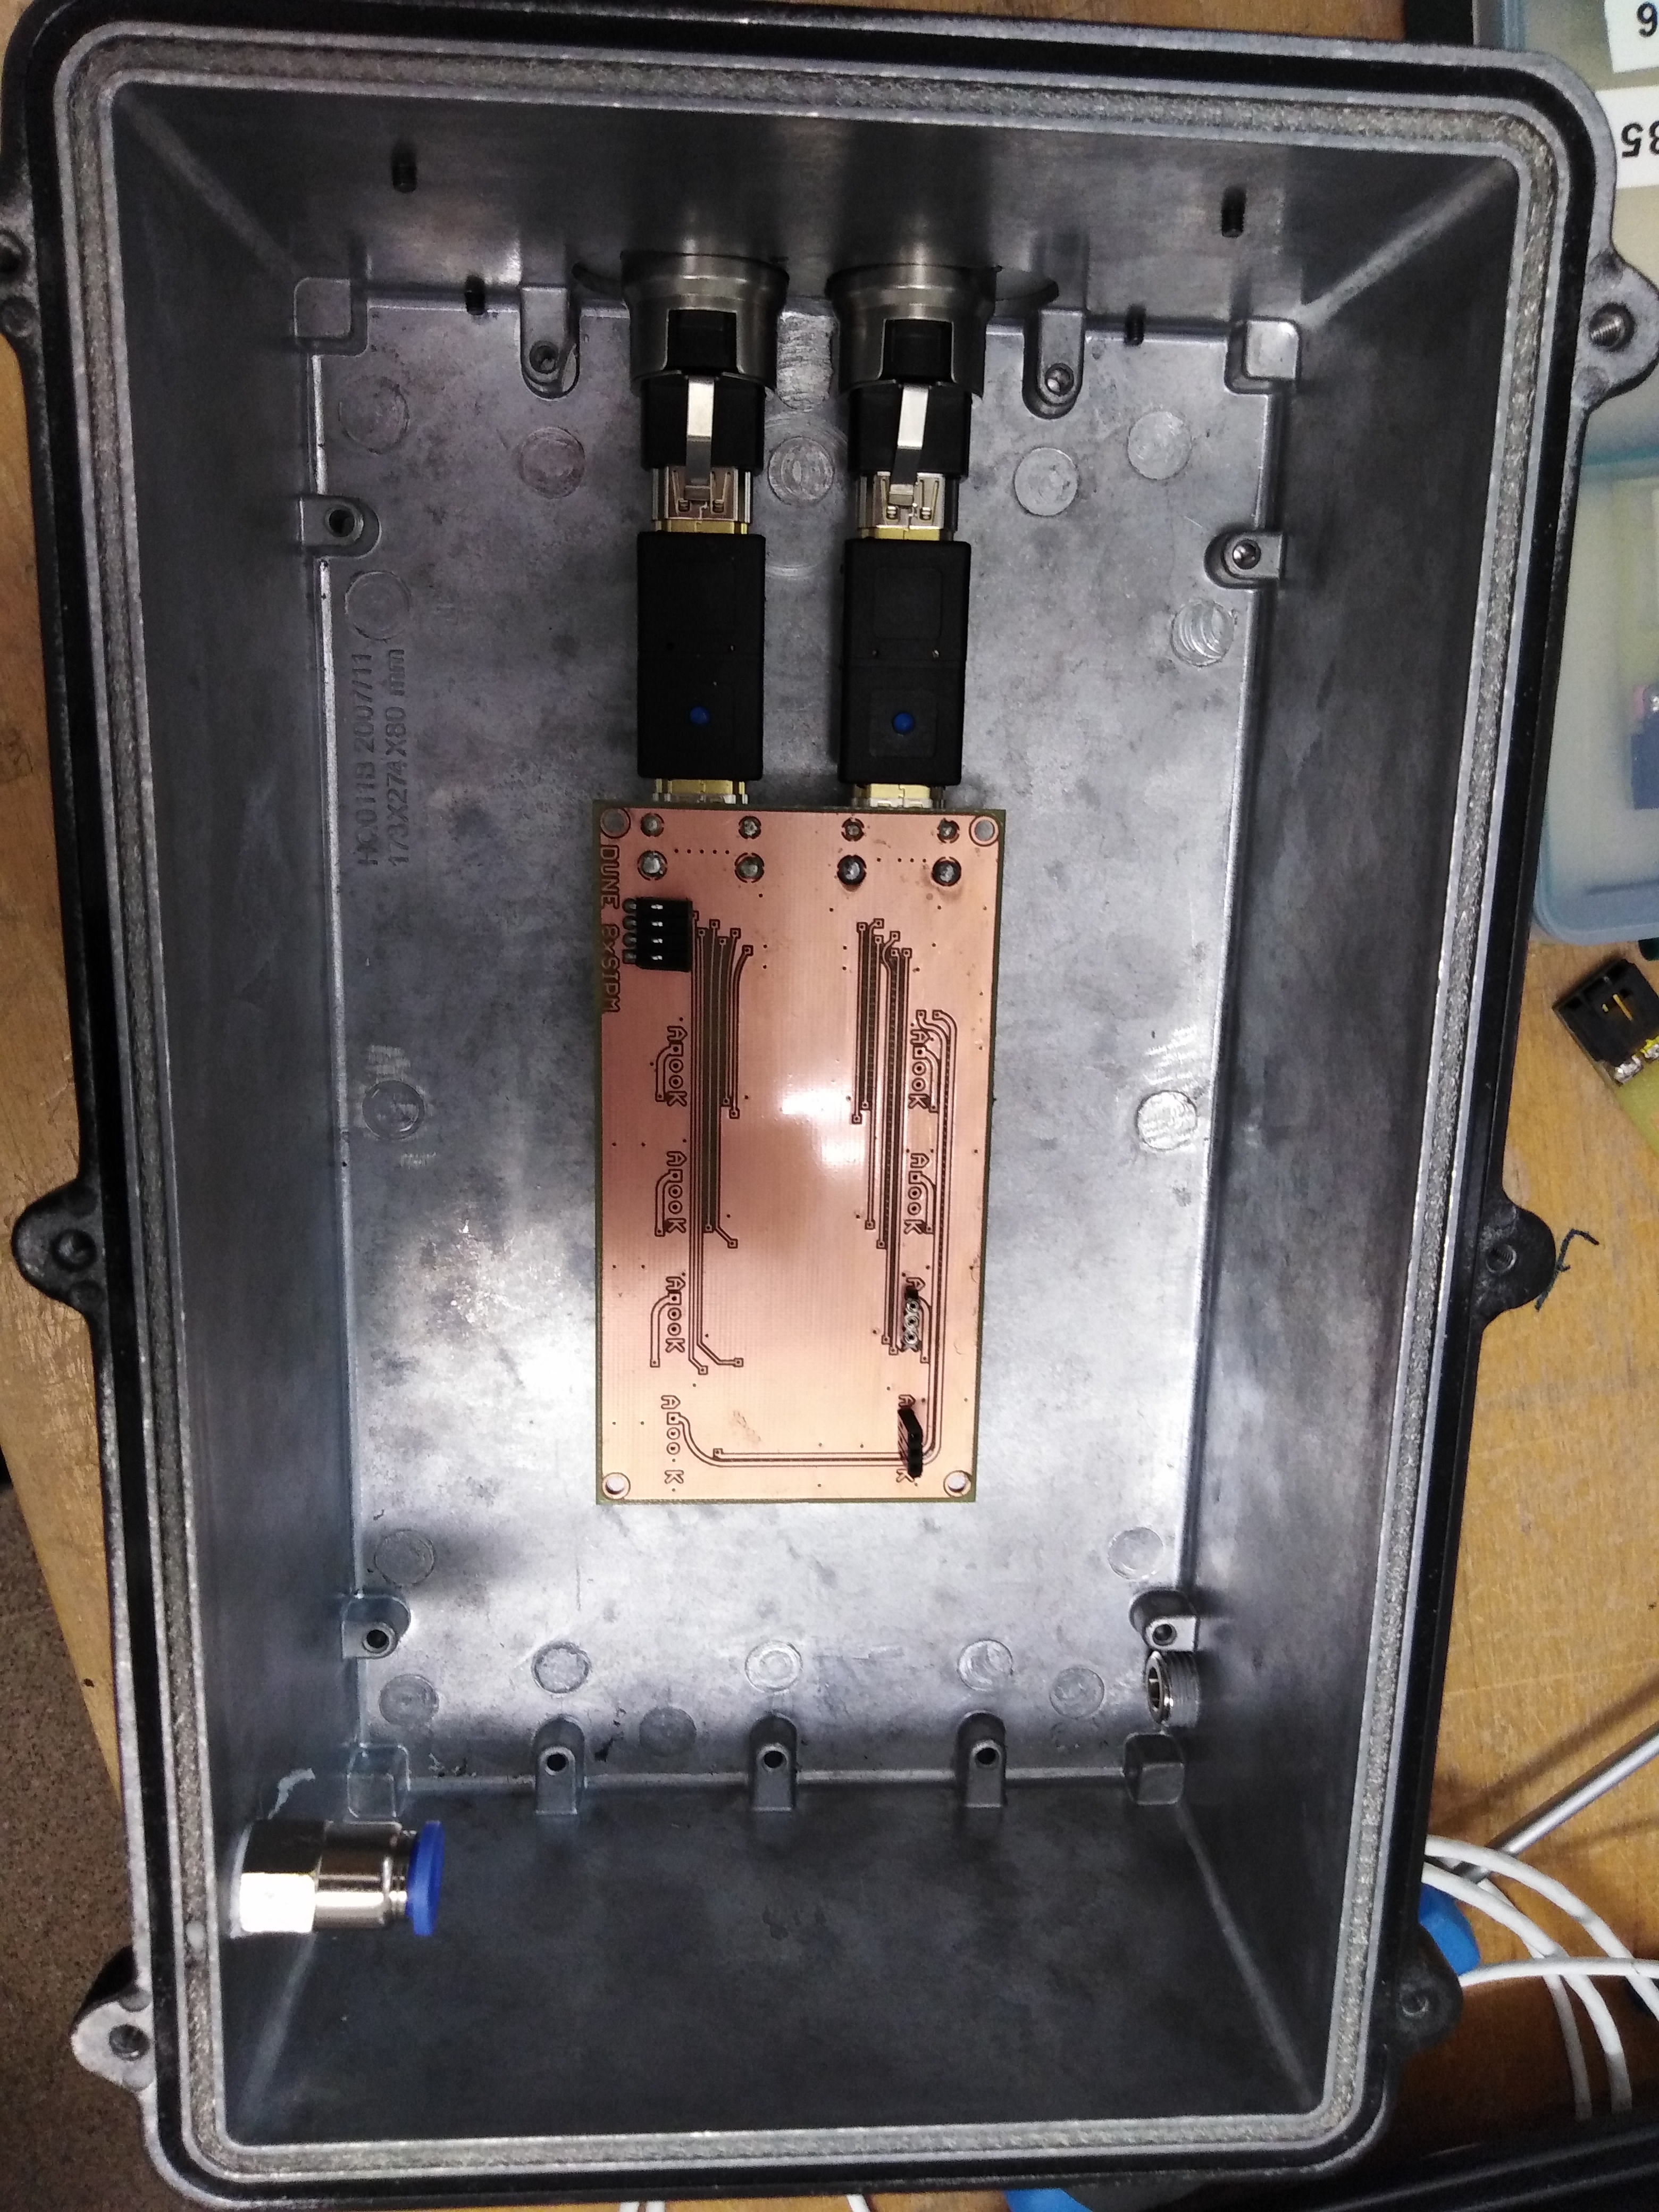
\includegraphics[width=\textwidth]{3DesignPrinciples/32Tritium_detector/PCB1_SiPM_Black_Box.jpg}  
    \caption{PCB 1 used to arrang 8 SiPMs and black box.\label{subfig:PCB1}}
    \end{subfigure}
    \hfill
    \begin{subfigure}[b]{0.45\textwidth}
    \centering
    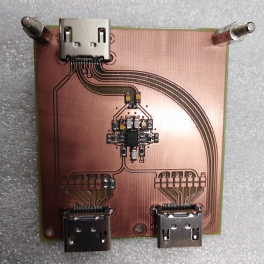
\includegraphics[width=\textwidth]{3DesignPrinciples/32Tritium_detector/PCB2_SIPMs.png}  
    \caption{PCB 2 used to sum and amplify the output signals of SiPMs.\label{subfig:PCB2}}
    \end{subfigure}
    \hfill
    \begin{subfigure}[b]{0.4\textwidth}
    \centering
    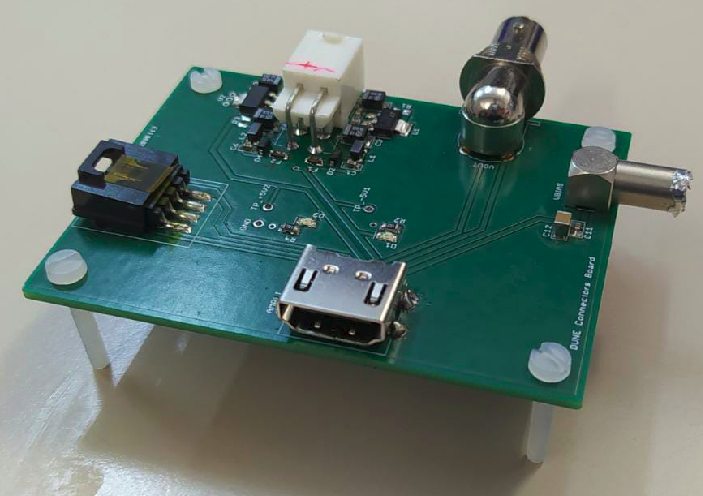
\includegraphics[width=\textwidth]{3DesignPrinciples/32Tritium_detector/PCB3_SiPMs.png}  
    \caption{PCB 3 used to rearrange the different singals of the system.\label{subfig:PCB3}}
    \end{subfigure}
    \hfill
    \begin{subfigure}[b]{0.5\textwidth}
    \centering
    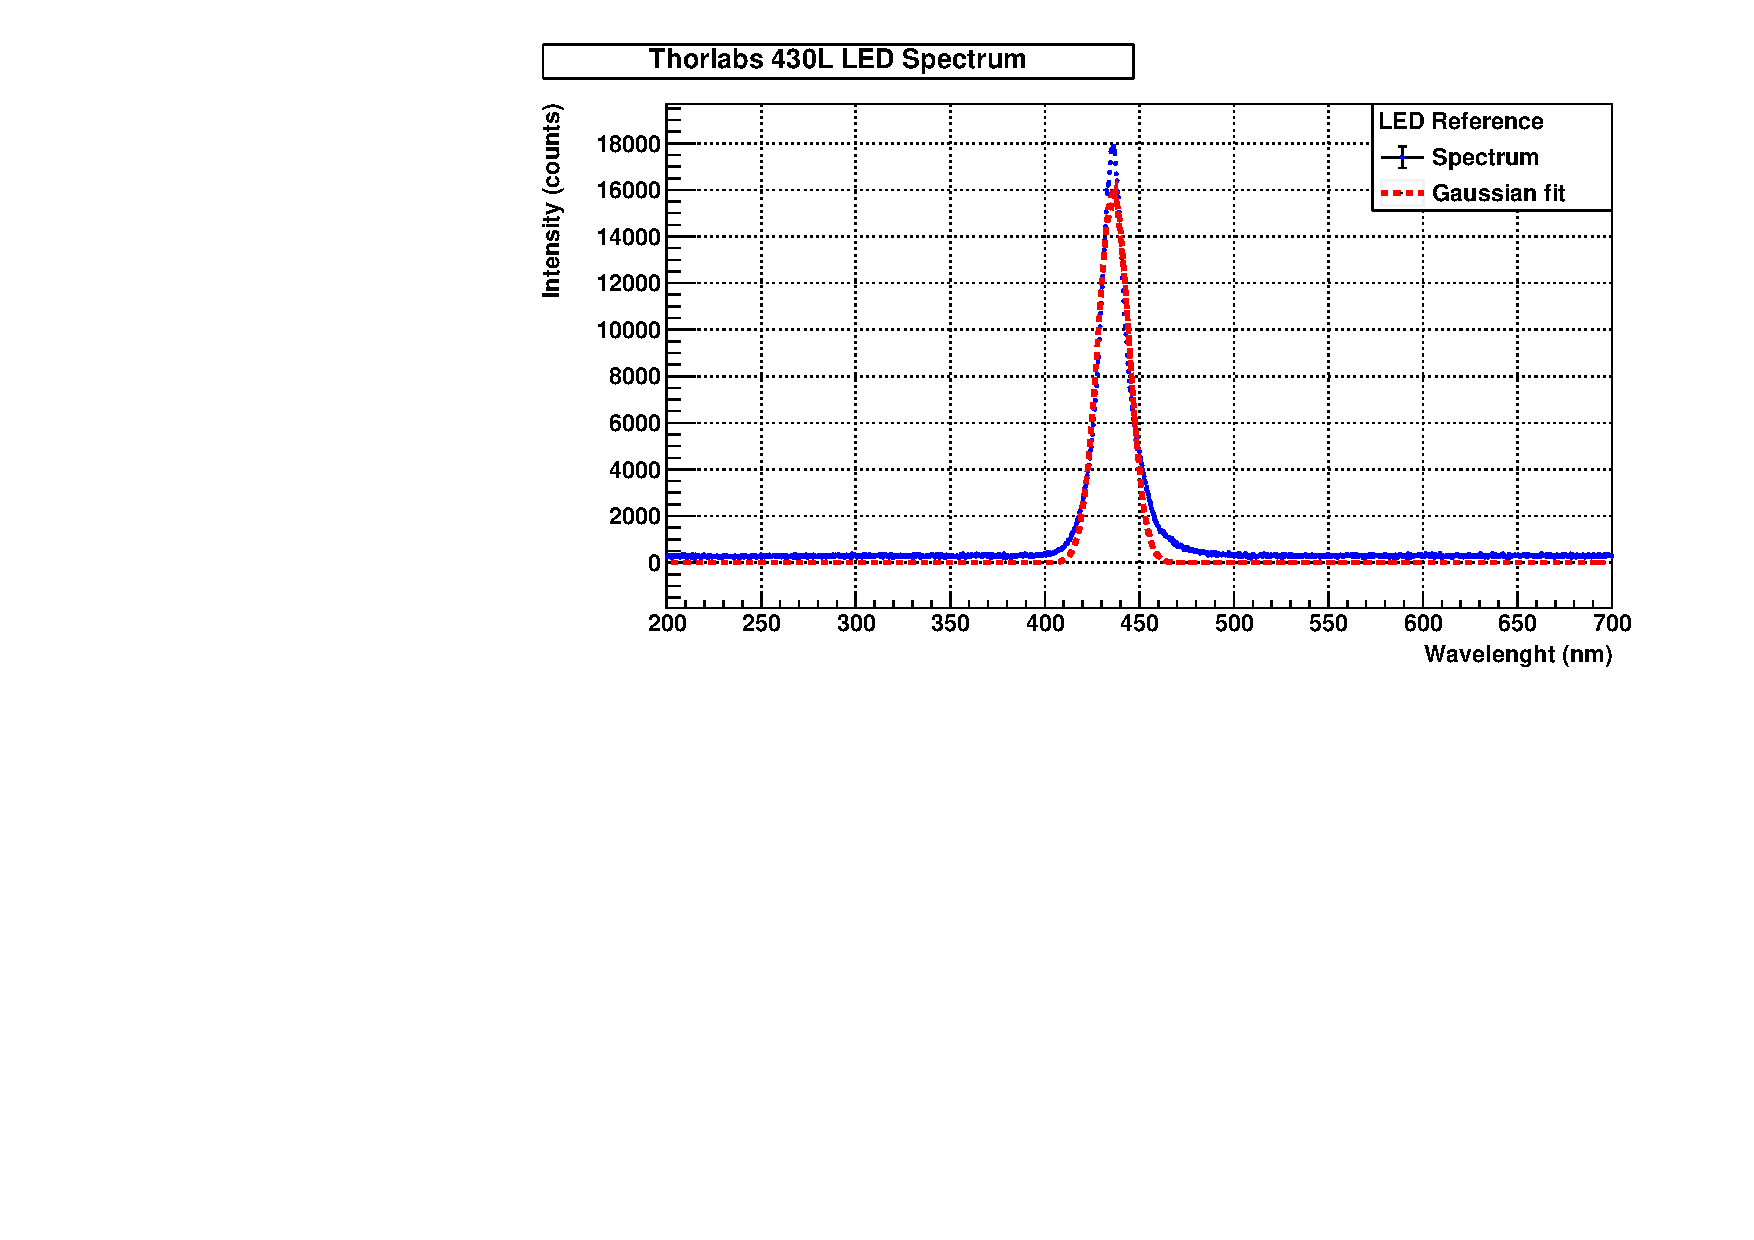
\includegraphics[width=\textwidth]{3DesignPrinciples/32Tritium_detector/LED_DUNE.pdf}  
    \caption{Emission spectrum of the LED.\label{subfig:LEDSpectrum}}
    \end{subfigure}
 \caption{Three PCBs used for the SiPM characterization and LED emission spectrum.}
 \label{fig:PCBs_LEDSpectrum}
\end{figure}

The output signal of the third PCB is connected to an oscilloscope, model MSO44X from Tektronix \cite{Oscilloscope} that records the data which are subsequently analized by ROOT\footnote{ROOT is a framework for data processing, based on C ++ and object-oriented technology, developed at CERN and widely used in nuclear and particle physics.}.